
\documentclass[10pt,a4paper]{article}

%%%%%%%%%%%%%%%%%%%%%%%%%%%%%%%%%%%%%%%%%%%%%%%%%%%%%%%%
%
% Packages and Theorem Environments

\usepackage{graphicx}
\usepackage{psfrag}
\usepackage{epsf}
\usepackage{amsmath,amsfonts,amssymb,latexsym}
\usepackage{enumitem}
\usepackage{algorithmic}
\usepackage{algorithm}
\usepackage[width=160mm,height=240mm,left=35mm,foot=10mm]{geometry}
\usepackage{xcolor}
\usepackage{url}
\usepackage{hyperref}
\usepackage{tikz}


\newcommand{\Cross}{\mathbin{\tikz [x=1.4ex,y=1.4ex,line width=.2ex] \draw (0,0) -- (1,1) (0,1) -- (1,0);}}%
\renewcommand{\theequation}{\thesection.\arabic{equation}}
\newcommand{\makeTiny}[1]{{\tiny #1}}
\newcommand{\work}{\tiny}
\newcommand{\ignore}[1]{}
\newcommand{\startClaims}{\setcounter{claim}{0}}
\newtheorem{theorem}{Theorem}[section]
\newtheorem{corollary}[theorem]{Corollary}
\newtheorem{lemma}[theorem]{Lemma}
\newtheorem{proposition}[theorem]{Proposition}
\newtheorem{conjecture}[theorem]{Conjecture}
\newtheorem{problem}[theorem]{Problem}
\newtheorem{question}[theorem]{Question}
\newtheorem{definition}[theorem]{Definition}
\newtheorem{task}[theorem]{Task}
\newtheorem{claim}{Claim}
\newtheorem{remark}[theorem]{Remark}
\newtheorem{observation}[theorem]{Observation}





\title{MATH 351 -- Assignment \#1\\
}

\author{Noah Alvard\\
591000449\\
Section 03}

\date{20200904}


%%%%%%%%%%%%%%%%%%%%%%%%%%%%%%%%%%%%%%%%%%%%%%%%%%%%%%%%
%
% Author's definitions


\newcommand{\NN}{\mathbb N}
\newcommand{\ZZ}{\mathbb Z}
\newcommand{\QQ}{\mathbb Q}
\newcommand{\RR}{\mathbb R}

\newcommand{\BB}{\mathcal B}
\newcommand{\ZT}{\mathcal Z}

\newcommand{\Cl}{\operatorname{Cl}}
\newcommand{\Bd}{\operatorname{Bd}}
\newcommand{\row}{\operatorname{row}}
\newcommand{\col}{\operatorname{col}}
\newcommand{\Span}{\operatorname{span}}
\newcommand{\convhull}{\operatorname{conv.hull}}
\newcommand{\tr}{\operatorname{tr}}

\newcommand{\diam}{\operatorname{diam}}

\begin{document}

\maketitle

\begin{center}
{\bf \large Part 2}
\end{center}

\subsection*{Problem 1}


\begin{figure}[h]
    \centering
    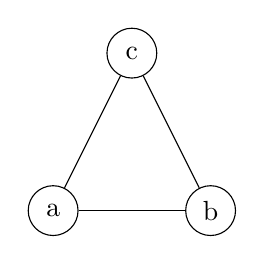
\begin{tikzpicture}[scale=0.2,every node/.style={circle,draw,inner sep=0pt,minimum width=18pt}]
    %
    \node (a) at (-5,0) {a};
    \node (b) at (5,0) {b};
    \node (c) at (0,10) {c};
    %
    \draw (a) edge (b);
    \draw (b) edge (c);
    \draw (c) edge (a);
    %
    \end{tikzpicture}
    %
    \caption{A graph with no odd vertices.}\label{GraphG}
\end{figure}

\begin{figure}[h]
    \centering
    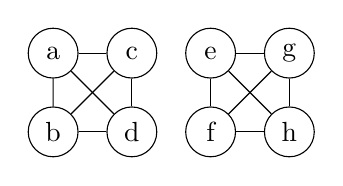
\begin{tikzpicture}[scale=0.2,every node/.style={circle,draw,inner sep=0pt,minimum width=18pt}]
    %
    \node (a) at (-10,5) {a};
    \node (b) at (-10,0) {b};
    \node (c) at (-5,5) {c};
    \node (d) at (-5,0) {d};

    \node (e) at (0,5) {e};
    \node (f) at (0,0) {f};
    \node (g) at (5,5) {g};
    \node (h) at (5,0) {h};
    %
    \draw (a) edge (b);
    \draw (b) edge (d);
    \draw (c) edge (a);
    \draw (d) edge (a);
    \draw (c) edge (d);
    \draw (b) edge (c);

    \draw (e) edge (f);
    \draw (f) edge (h);
    \draw (g) edge (e);
    \draw (h) edge (e);
    \draw (g) edge (h);
    \draw (f) edge (g);
    %
    \end{tikzpicture}
    %
    \caption{A noncomplete graph where all vertices have degree 3}\label{GraphG}
\end{figure}


\begin{figure}[h]
    \centering
    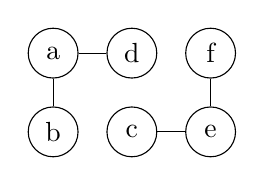
\begin{tikzpicture}[scale=0.2,every node/.style={circle,draw,inner sep=0pt,minimum width=18pt}]
    %
    \node (a) at (-5,5) {a};
    \node (b) at (-5,0) {b};
    \node (c) at (0,0) {c};
    \node (d) at (0,5) {d};
    \node (e) at (5,0) {e};
    \node (f) at (5,5) {f};
    %
    \draw (a) edge (b);
    \draw (a) edge (d);
    \draw (f) edge (e);
    \draw (e) edge (c);
    %
    \end{tikzpicture}
    %
    \caption{A graph of order at least 5 with where the degree of adjacent vertices is not equal}\label{GraphG}
\end{figure}
\pagebreak
\begin{figure}[h]
    \centering
    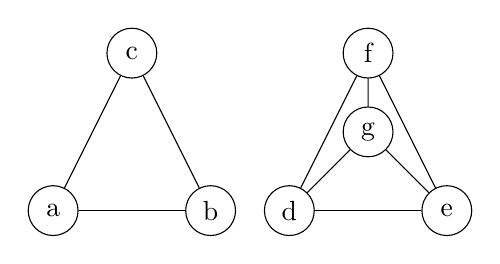
\begin{tikzpicture}[scale=0.2,every node/.style={circle,draw,inner sep=0pt,minimum width=18pt}]
    %
    \node (a) at (-5,0) {a};
    \node (b) at (5,0) {b};
    \node (c) at (0,10) {c};

    \node (d) at (10,0) {d};
    \node (e) at (20,0) {e};
    \node (f) at (15,10) {f};
    \node (g) at (15,5) {g};
    %
    \draw (a) edge (b);
    \draw (b) edge (c);
    \draw (c) edge (a);
    
    \draw (d) edge (e);
    \draw (e) edge (f);
    \draw (f) edge (d);
    \draw (g) edge (d);
    \draw (g) edge (e);
    \draw (g) edge (f);
    %
    \end{tikzpicture}
    %
    \caption{A graph of order at least 5 with where the degree of nonadjacent vertices is not equal}\label{GraphG}
\end{figure}

\subsection*{Problem 2}

A graph is bipartite if it's vertices can be split into two distinct groups where there are no edges between the vertices in the group.
The property of G directly lends itself to G being bipartite as it describes the two groups. The first being of all the odd vertices, and
the second being of all the even vertices. There can be no connections between vertices within the group due to the restraint of the property given.

By the property, G must also have an even size (for my benefit, an even number of edges). Because we already know that G is bipartite,
we know that there exists a group of only even vertices. As the only possible edges are between the even vertex group and the odd vertex group, and 
the the edges coming out of the even group are the only edges in the graph, so the size of the graph is even.

\subsection*{Problem 3}

Using theorem 2.10, the sequence of 7, 6, 5, 4, 3, 2, 1, x is graphable for the value of x = 4.

\subsection*{Problem 4}

Due to G being bipartite, the adjacency matrix $A$ is very simple. The two groups will be refered two as E and F.
From $Uv_0$ to $Uv_r$ and $Wv_{r+1}$ to $Wv_{2r}$, the values are 1
From $Uv_{r+1}$ to $Uv_{2r}$ and $Wv_0$ to $Wv_r$ the avlues are 1.
In all other spaces the values are 0.
This shows that all all the vertices between the groups are adjacent, but none of the vertices in the group are adjacent.
The values in the matrix $A^n$ represent how many walks of length n are between two vertices.

So $A^2$ is for walks of length 2. Knowing that the graph is bypartite, and that the two groups each
have $r$ vertices. To get from vertex u to any other vertex you have to go from the vertex, to the other side (1 of r choices), and back.
This means that the matrix is inverted and multiplied by $r^n$.
From $Uv_0$ to $Uv_r$ and $Wv_0$ to $Wv_r$, the values are $r^2$.
From $Uv_{r+1}$ to $Uv_{2r}$ and $Wv_{r+1}$ to $Wv_{2r}$ the avlues are $r^2$.
In all other spaces the values are 0.

This pattern repeats for higher values of n as well. The two quadrants of values flipping for odd/even values of n, and the values being in those quadrants scalling with $r^n$

\begin{center}
    {\bf \large Part 3}
    \end{center}

\subsection*{Problem 5}

Prove that if G is a graph of order n such that $\Delta(G) + \delta(G) \geq n - 1$, then G
is connected AND diam(G) $\leq$ 4. Show that the bound $n - 1$ is sharp.

Order n, means n vertices
if the max degree is x, and the min degree is y
and x + y >= n-1

n is 5
max is 2
min is 1
2+1 !>= n-1

I'm confused


\end{document} 




















